\documentclass[10pt]{beamer}
\usepackage{ngerman}
\usepackage[utf8]{inputenc}
\usepackage[]{amsmath}
\usepackage{amsthm}
\usepackage[ngerman]{babel}
\usepackage[T1]{fontenc}
\usepackage{lmodern}
\usepackage{graphicx}
\usepackage{algorithm}
\usepackage{algpseudocode}

\newtheorem{satz}{Satz}

\usetheme{default}
\useinnertheme{circles}
\setbeamertemplate{bibliography item}[text]

\title{Analyse des OpenPGP Web of Trust}
\author{Alexander Ulrich \\ \texttt{ulricha@informatik.uni-tuebingen.de}}
\institute{Wilhelm-Schickard-Institut für Informatik\\
          Universität Tübingen}

\date{Abschlussvortrag Studienarbeit\\23.06.2010}

\begin{document}

\begin{frame}
  \titlepage
\end{frame}
\begin{frame}
  \frametitle{Motivation}
  \begin{itemize}
  \item In den letzten Jahren steigende Verf\"ugbarkeit von Daten
    \"uber gro{\ss}e, komplexe Netzwerke (z.B. technologische,
    soziale, biologische)
  \item Analyse der Struktur dieser Netzwerke kann interessante
    Einblicke in die Mechanismen der zugrundeliegenden Systeme liefern
  \item OpenPGP (PGP/GnuPG): praktikables und weit verbreitetes Paket
    f\"ur Verschl\"usselung und Authentifizierung, insbesondere von E-Mail
  \item Web of Trust: dezentraler Authentifizierungsmechanismus f\"ur
    Schl\"ussel liefert komplexes Netzwerk
  \item verf\"ugbare Datens\"atze \"uber das Web of Trust sind
    veraltet oder fehlerhaft
  \item bisherige Arbeiten beruhen meist auf sehr alten Daten oder
    haben sich nur am Rand mit der Netzwerkstruktur besch\"aftigt
  \end{itemize}
\end{frame}

\begin{frame}
  \frametitle{Web of Trust}
  \begin{itemize}
  \item Public-Key-Kryptographie: Verteilung von (\"offentlichen)
    Schl\"usseln \"uber unsichere Kan\"ale
  \item Notwendig: \"Uberpr\"ufung der \emph{Authentizit\"at} von
    Schl\"usseln
  \item Digitale Signaturen auf Schl\"usseln nach \"Uberpr\"ufung der
    Identit\"at
  \item X.509: zentrale \emph{Certificate Authorities} (CA)
  \item Web of Trust: Jeder Teilnehmer  kann als CA fungieren, jeder
    Teilnehmer entscheidet selbst, welchen CAs er \emph{vertraut}
  \item Signaturen aller Teilnehmer ergeben einen gerichteten Graphen
  \item Aufbau von Signaturketten: jedem Kettenglied muss vertraut
    werden
  \item Hypothese: Signaturen spiegeln \emph{soziale Beziehungen}
    wieder $\Rightarrow$ soziales Netzwerk
  \item Keysigning-Parties
  \end{itemize}
\end{frame}

\begin{frame}
  \frametitle{Fragestellung}
  \begin{itemize}
  \item Wie ist das Netzwerk insgesamt aufgebaut?
  \item Verf\"ugt das Netzwerk \"uber eine (regelm\"a{\ss}ige)
    \emph{Struktur} oder ist es vollst\"andig chaotisch?
  \item Inwiefern spiegelt die Graphenstruktur die zugrundeliegenden
    Mechanismen (Signierung von Schl\"usseln) wieder?
  \item Wie stark wird das System Web of Trust \"uberhaupt benutzt?
  \item Wie gut erf\"ullt es seinen Zweck?
  \end{itemize}
\end{frame}

\begin{frame}
  \frametitle{\"Ubersicht \"uber die Arbeit}
  \begin{enumerate}
  \item Implementierung der Datenextraktion aus Schl\"usseldatenbank
  \item Analyse der Struktur des Graphen auf verschiedenen Ebenen
    \begin{itemize}
    \item Struktur der starken Zusammenhangskomponenten
    \item Gegenseitigkeit von Kanten
    \item Clustering und Small-World
    \item Gradverteilung
    \item Community-Struktur
    \end{itemize}
  \item Sonstige Netzwerkeigenschaften
    \begin{itemize}
    \item Robustheit
    \item N\"utzlichkeit
    \end{itemize}
  \item Schl\"usseleigenschaften
    \begin{itemize}
    \item Zeitliche Entwicklung des Schl\"usselbestandes
    \item Verwendung von Public-Key-Algorithmen und Hashalgorithmen
\end{itemize}
  \end{enumerate}
\end{frame}

\begin{frame}
  \frametitle{Software}
  Extraktion
  \begin{itemize}
  \item Integriert in SKS-Keyserver (OCaml, $\approx 1200$ LOC)
  \item Reduzierung von OpenPGP-Schl\"usseln auf interessante Daten
  \item Daten in SQL-Datenbank abgelegt
  \item speichert komplette Geschichte: Zeitpunkte von Schl\"ussel-
    und Signaturerzeugung, Ablaufdatum, Widerrufsdatum
  \item Zus\"atzliche Daten: Public-Key-Algorithmus und
    Hashalgorithmus, Schl\"ussell\"angen, UserIDs
  \end{itemize}

Auswertung
\begin{itemize}
\item Sammlung von Kommandozeilenwerkzeugen (OCaml, $\approx 3800$
  LOC)
\item All-pair-shortest-path und Betweeness centrality auf MPI-Cluster
\end{itemize}
\end{frame}

\begin{frame}
  \frametitle{Datensatz}
  \begin{itemize}
  \item Datenbank: 2700000 Schl\"ussel, 1100000 Signaturen
  \item 410000 Schl\"ussel abgelaufen, 100000 widerrufen, 50000 defekt
  \item Komplett unvernetzte Schl\"ussel entfernt
  \item Graph mit 325000 Knoten, 817000 Kanten
  \item Gro{\ss}teil der verf\"ugbaren Schl\"ussel ist nicht
    verifizierbar, kann keine Signaturketten verwenden
  \item unbekannte Anzahl von \emph{nicht-\"offentlichen} Signaturen
  \item Keine Aussage \"uber \emph{aktuelle} Anzahl von PGP-Benutzern
    m\"oglich
  \end{itemize}
\end{frame}

\begin{frame}
  \frametitle{Zusammenhangskomponenten}
  Bekannt: Eine gigantische starke Zusammenhangskomponente (MSCC) mit
  ca. 45000 Knoten. Aber: Wie ist der Rest strukturiert?

  \begin{itemize}
  \item ca. 240000 Komponenten
  \item Deutlich \"uber 100000 mit Gr\"o{\ss}e 1, 10000-20000
    Knotenpaare, wenige zwischen 10 und 100
  \item Einzelne Knoten oder sehr kleine Cluster, die einzelne Kanten
    zu anderen Komponenten haben
  \item Komponenten untereinander kaum vernetzt
  \item \emph{bow tie}: in 18000 Knoten, out 92000 Knoten
  \end{itemize}

  $\Rightarrow$ Nennenswerte Signaturaktivit\"at nur in der MSCC,
  f\"ur restliche Schl\"ussel ist das Web of Trust kaum benutzbar.
\vspace{0.5cm}

  Rest der Arbeit konzentriert sich auf MSCC: 45000 Knoten, 443000
  Kanten (Capkun 2001: 12000 Knoten).
  
\end{frame}

\begin{frame}
  \frametitle{Strukturelle Merkmale}
  \begin{description}
  \item[Gegenseitigkeit]
    \begin{itemize}
    \item ca. 50\% aller Kanten haben eine Gegenkante 
    \item Erkl\"arung: Signierung normalerweise beidseitig
    \item positive Korrelation zwischen ein- und ausgehendem Grad
    \end{itemize}
  \item[Small-World] 
    \begin{itemize}
    \item Geringe charakt. Distanz $\approx 12$ $\Rightarrow$
      Small-World-Effekt
      \item Interessant aufgrund weltweiter geographischer Verteilung der
        Teilnehmer
      \item Radius 16, Durchmesser 36
    \end{itemize}
  \item[Clustering] 
    \begin{itemize}
    \item hoher Clustering coefficient $C = 0,460$ (configuration
      model $C = 0,013$)
    \item hohes Ma{\ss} an Clustering charakteristisch f\"ur soziale
      Netzwerke (Newman 2003)
    \item Grund: Community-Struktur
    \end{itemize}
  \end{description}
\end{frame}

\begin{frame}
  \frametitle{Gradverteilung (1)}
  Durchschnittlicher ausgehender Grad 9,29
  \begin{figure}
    \centering
    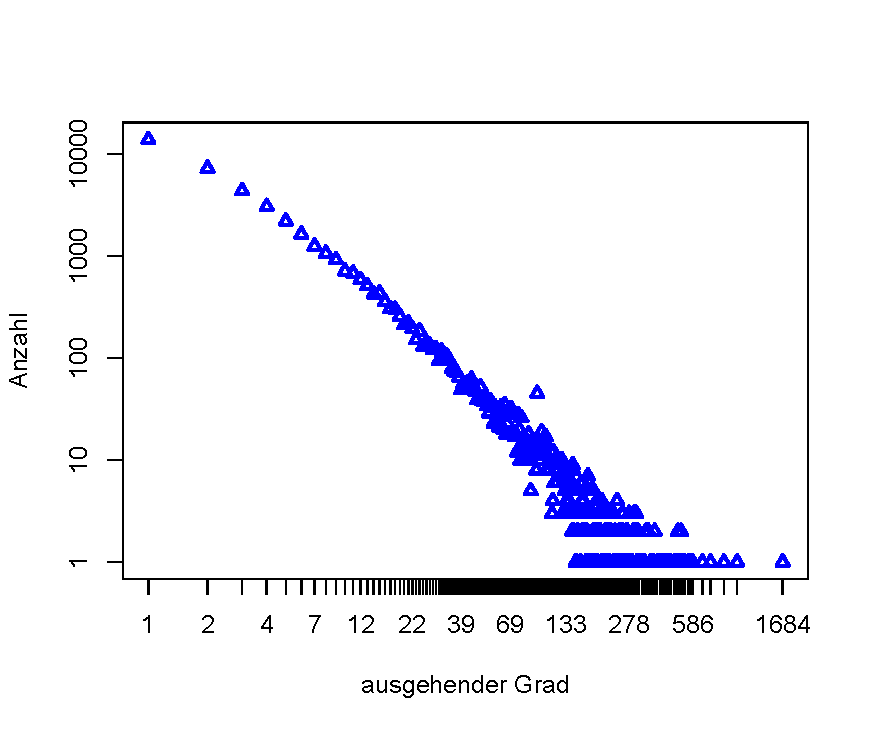
\includegraphics[scale=0.3]{../ausarbeitung/images/outdegree-dist.pdf}
  \end{figure}
\begin{itemize}
\item Sehr inhomogene Verteilung, Durchschnitt ist wenig
aussagekr\"aftig.
\item Ann\"ahernd gerade auf log-log-Plot $\Rightarrow$ Power-Law?
\end{itemize}
\end{frame}

\begin{frame}
  \frametitle{Gradverteilung (2)}
  \begin{itemize}
  \item Bestimmung des Exponenten: keine lineare Regression
  \item Stattdessen Maximum-Likelihood-Methode (Clauset 2009):
    $x_{min} \approx 84$, $\alpha = 2,35$
  \item \"Uberpr\"ufung der Anpassungsg\"ute (Kolmogorov-Smirnov) schlie{\ss}t power law
    aus
  \item Zentrales Merkmal in Literatur zu skalenfreien Netzwerken:
    Hub-Struktur, "robust yet fragile" (Albert 2000)
  \item Power law weder hinreichend noch notwendig f\"ur Hub-Struktur
    (Li 2005)
  \item Verteilung mit hoher Variabilit\"at, gut vernetzte Knoten
    prim\"ar mit anderen gut vernetzten Knoten verbunden
  \item Tats\"achlich: (schwache) positive Korrelation zwischen Graden
    benachbarter Knoten
  \end{itemize}
\end{frame}

\begin{frame}
  \frametitle{Robustheit (1)}
  \begin{figure}
    \centering
    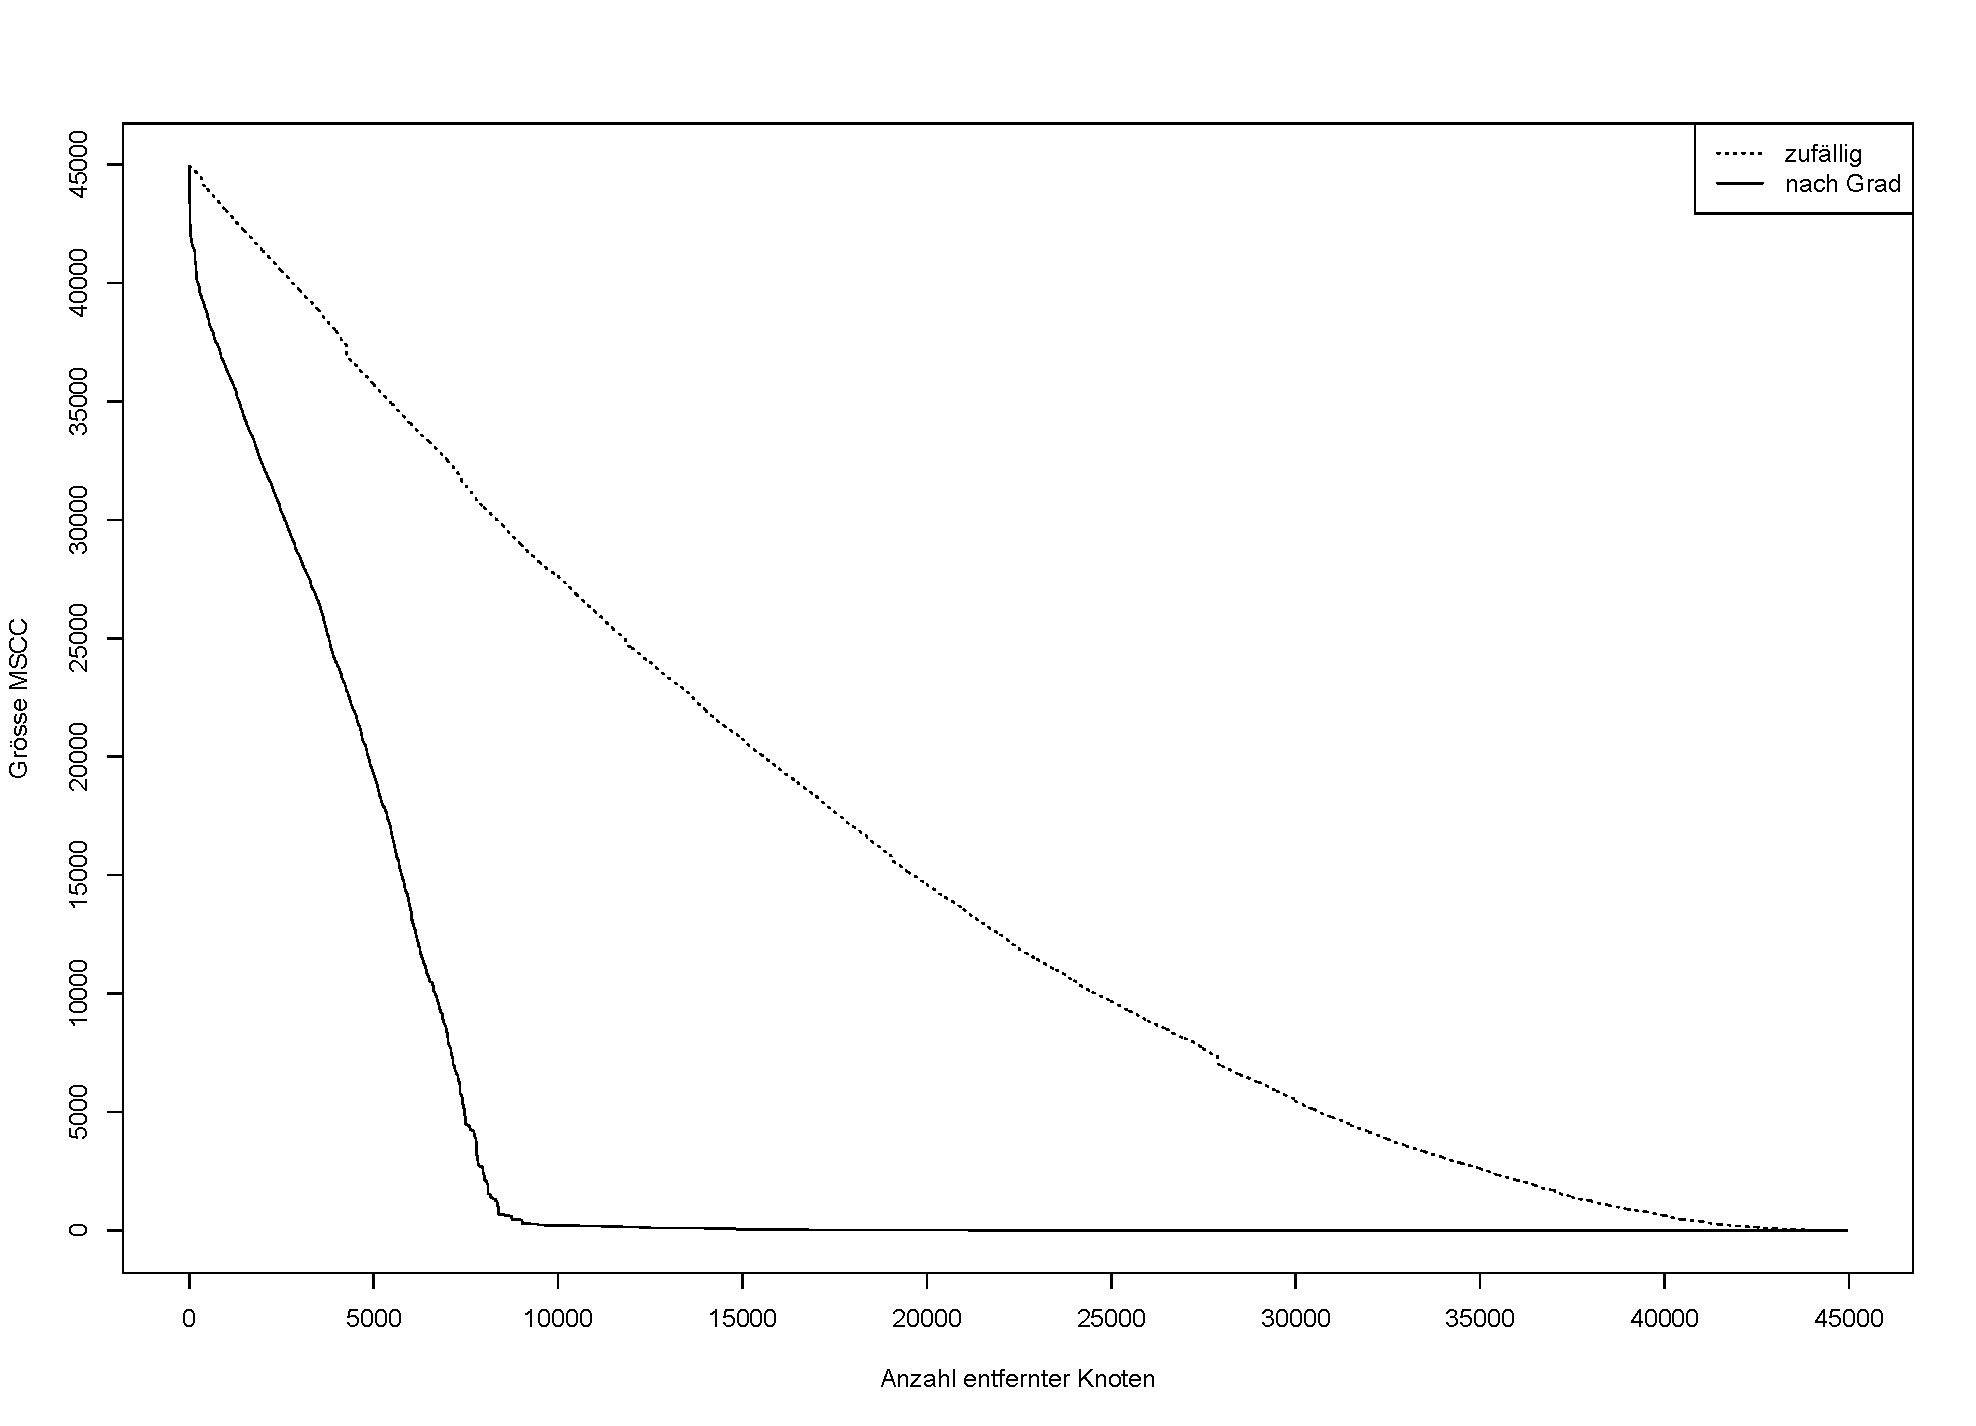
\includegraphics[scale=0.3]{../ausarbeitung/images/without.pdf}
  \end{figure}
\end{frame}

\begin{frame}
  \frametitle{Robustheit (2)}
  \begin{description}
  \item[zuf\"allige Sch\"adigung] Ablaufsdatum, Passphrase
    vergessen, neuer Schl\"ussel\dots
  \item[gezielter Angriff] Kompromittierung
\end{description}
\begin{itemize}
  \item Netzwerk ist sehr robust gegen Sch\"adigung
  \item Netzwerk ist \"uberraschend robust gegen gezielten Angriff,
    kein rapider Zerfall
  \item $\Rightarrow$ Zusammenhalt h\"angt nicht von wenigen gut
    vernetzten Knoten ab, keine ausgepr\"agte Hub-Struktur
  \item charakteristische Distanz/Durchmesser nicht betrachtet
  \item Knoten mit h\"ochstem Grad sind nicht unbedingt die
    \emph{zentralsten} Knoten
  \end{itemize}
  
\end{frame}

\begin{frame}
  \frametitle{N\"utzlichkeit (1)}
  \begin{itemize}
  \item Mindestvorraussetzung f\"ur Verifizierbarkeit: Signaturkette
    $\Rightarrow$ Pfad
  \item Wichtige Einschr\"ankung: maximale Pfadl\"ange {\bf 5}
  \item Zus\"atzlich: \emph{Vertrauen} in jedes Glied der
    Signaturkette
  \item Erhebliche Einschr\"ankung f\"ur Knoten mit Grad 1
    (ein-/ausgehend): keine Redundanz
  \item Radius 16, durchschnittliche Eccentricity $\approx 28$, durchschnittliche Distanz 12
  \item Je l\"anger die Kette desto mehr Vertrauen ist notwendig
    $\Rightarrow$ betrachte auch k\"urzere Ketten
  \item $h$-Nachbarschaften ($h=1, \dots, 5$)
  \end{itemize}
  
\end{frame}

\begin{frame}
  \frametitle{N\"utzlichkeit (2)}
  \begin{figure}
    \centering
    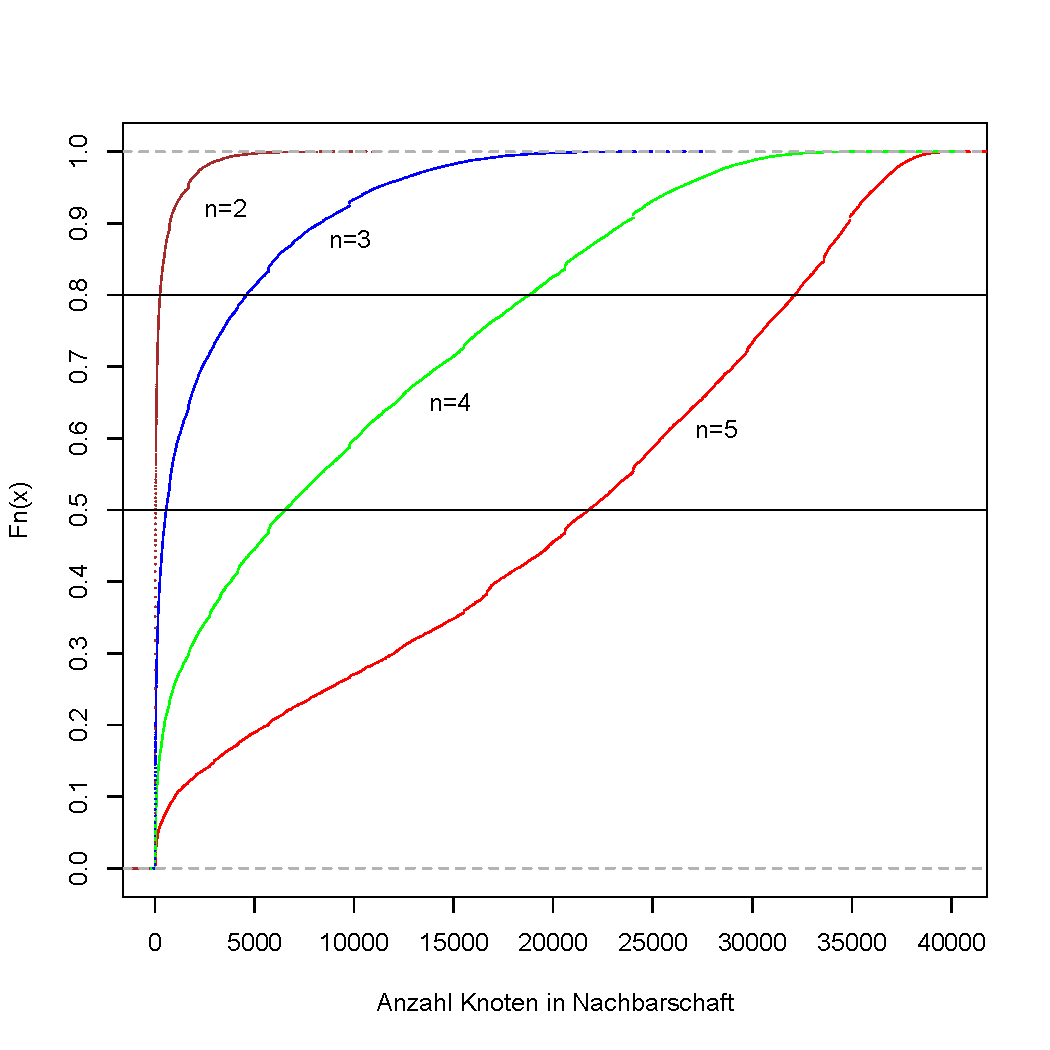
\includegraphics[scale=0.45]{../ausarbeitung/images/neighbourhood-cdf.pdf}
  \end{figure}
\end{frame}


\begin{frame}
  \frametitle{Zusammenfassung}
  \begin{itemize}
  \item Extraktionssoftware und Datensatz
  \item Je n\"aher das Netzwerk betrachtet wird, desto kleiner scheint
    der aktive Teil
  \item charakteristische Merkmale eines sozialen Netzwerks
  \item recht robust gegen\"uber Fehlern und gezielten Angriffen
  \item Erreichbarkeit bei kleinen Pfadl\"angen ist f\"ur die meisten
    Knoten gering
  \end{itemize}
\end{frame}
% \begin{frame}
%   Danke für eure Aufmerksamkeit.\\[1cm]

%   Fragen? Anmerkungen?
% \end{frame}

\begin{frame}
  \begin{center}
    {\Huge ?}
  \end{center}
  
\end{frame}

\begin{frame}
\nocite{PhysRevE.68.036122}
\nocite{Clauset2009}
\nocite{Albert2000}
\nocite{Fortunato2010}
  \frametitle{Literatur}
  
  {\small
  \bibliographystyle{plain}
  \bibliography{diplarb}
}
\end{frame}

\begin{frame}
  \frametitle{Communities (1)}
  \begin{itemize}
  \item Individuen in sozialen Netzwerken neigen zu Gruppenbildung:
    famili\"ar, freundschaftlich, gemeinsame Interessen,
    professionell\dots
  \item Communities: Gruppen von Knoten, die untereinander \"uber
    viele Kanten verf\"ugen, nach ausserhalb nur wenige Kanten
    (Fortunato 2010)
  \item Hypothese: Signaturentstehung wird von sozialen Beziehungen
    und Keysigning-Parties bestimmt
  \item Frage: hat der Graph eine ausgepr\"agte Community-Struktur?
  \item Frage: L\"asst sich f\"ur Communities entscheiden, wie sie
    entstanden sind?
  \item Kriterien: SLD aus UserIDs (Organisation, Land), zeitliche
    Korrelation der Signaturen (Keysigning-Party)
  \end{itemize}
  
\end{frame}

\begin{frame}
  \frametitle{Communities (2)}
  \begin{figure}
    \centering
  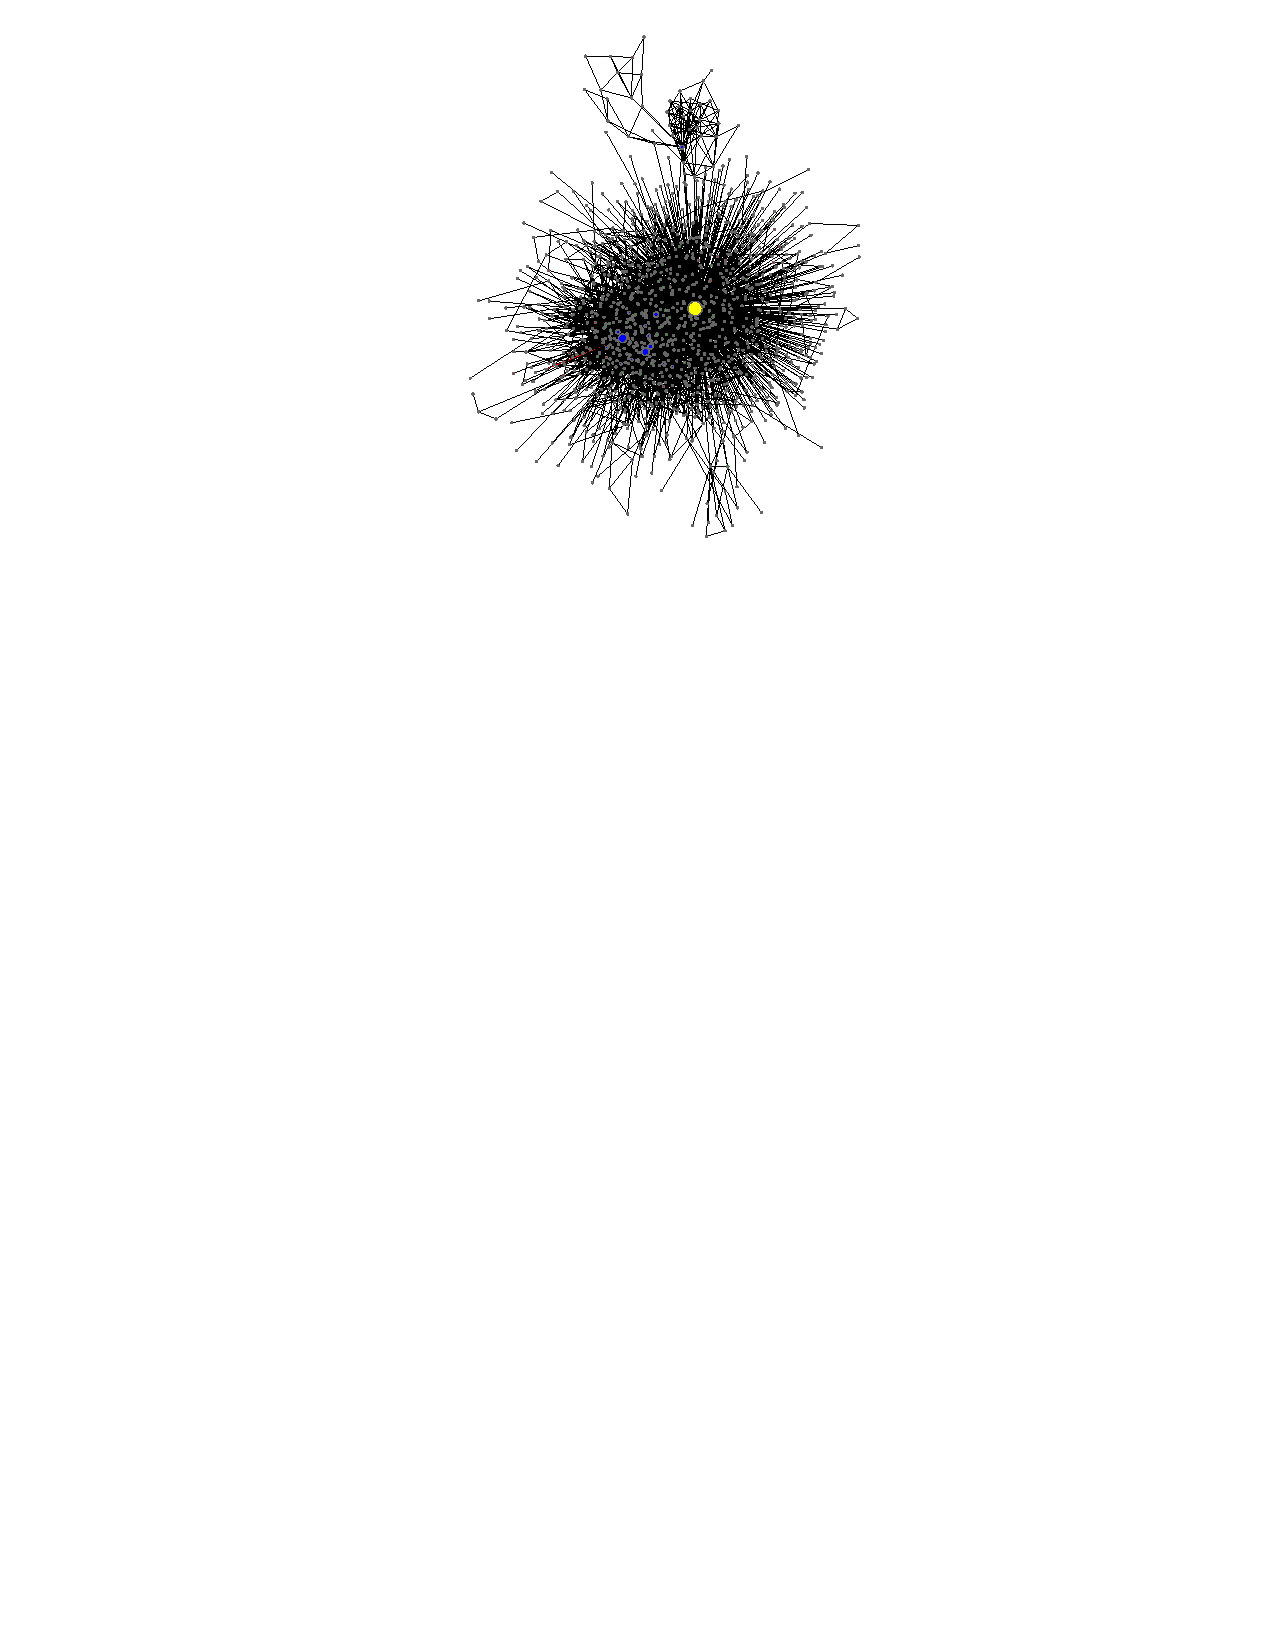
\includegraphics[scale=1.1,angle=90]{../ausarbeitung/images/metagraph-copra1-minsize5.pdf}
   \caption{Struktur der Communities gr\"o{\ss}er 5} 
  \end{figure}
  
\end{frame}

\begin{frame}
  \frametitle{Communities (3)}
  \begin{itemize}
  \item 1421 Communities gr\"osser 3, stark inhomogene Verteilung
  \item Aufteilung gibt die Struktur des Netzwerkes gut wieder
    (Modularity $Q=0,780$) $\Rightarrow$ tats\"achlich ausgepr\"agte
    Community-Struktur
  \item eine gigantische Community, Rest tendenziell sternf\"ormig
    angeordnet
  \item Fast alle Communities sind einem Land zuordnenbar
  \item Zuordnung zu SLDs funktioniert nur bei kleineren Communities,
    nicht bei besonders vielen (Ausnahmen: apache.org (436, 48\%),
    cert.org (97, 70\%), \dots)
  \item Zeitliche Korrelation bei 40\% der Communities,
    haupts\"achlich kleineren
  \end{itemize}
  
\end{frame}

\begin{frame}
  \frametitle{Communities (4)}

  \begin{itemize}
  \item Annahme nicht widerlegt
  \item Methoden zu primitiv, um Entstehungsmechanismus zu erkl\"aren
  \item Sehr beschr\"ankte Daten \"uber soziale Gruppenzugeh\"origkeit
    (nur UserIDs)
  \item Je aktiver die Teilnehmer, desto unsch\"arfer wird das Bild
    $\Rightarrow$ Communities verschmelzen
  \item Beispiel: Gr\"osste Community ist intern sehr dicht
  \item Zugeh\"origkeit zu \emph{einer} Gruppe ist oft nicht
    entscheidend
  \item Beispiel: Debian
  \end{itemize}

  
  M\"oglicherweise interessant:
  \begin{itemize}
  \item Anhand der Entstehungsgeschichte
    des Netzwerks Entwicklungsdynamik der Communities nachvollziehen
  \item Untersuchen, wie Communities untereinander in Bezug auf
    nationale/geographische Zuordnung vernetzt sind
  \end{itemize}
  
\end{frame}

\end{document}
